\documentclass{beamer}
\mode<presentation>{\usetheme{Copenhagen}}

\usepackage[tikz]{bclogo}
\usepackage{mathtools}
\presetkeys{bclogo}{
	ombre=true,
	epBord=3,
	couleur = blue!15!white,
	couleurBord = red,
	arrondi = 0.2,
	logo=\bctrombone
}{}
\usepackage{etoolbox}
\makeatletter
\patchcmd{\insertverticalnavigation}%
{\ifx\beamer@nav@css\beamer@hidetext{\usebeamertemplate{section in sidebar}}\else{\usebeamertemplate{section in sidebar shaded}}\fi}%
{{\usebeamertemplate{section in sidebar}}}{}{}
\makeatother
\title{Machine Learning in Astronomy}
\author{Reza Monadi}
\institute{UC Riverside}
\date{May 14, 2020}
\begin{document}
	
	\frame{\titlepage}
	
	\begin{frame}
	\centering
	
\includegraphics[height=6cm, angle=0,origin=c]{ml.jpg}
	\tiny{credit: 365datascience.com}
	
\end{frame}

	
\section{Outline}
\frame{
	\begin{itemize}
		\uncover<1->{\item How astronomy is tied to \textbf{BIG DATA}?}
		\uncover<2->{\item What is  \textbf{ML}?}
		\uncover<3->{\item How to implement \textbf{ML} in astronomy? }
		\uncover<4->{\item How \textbf{ML} helps \textbf{SKA}?}
		\uncover<5->{\item What are the pitfalls of \textbf{ML} in astronomy?}
	\end{itemize}
	}

\section{Big Data}
\subsection{Definition of BIG DATA}{
	\frame{\frametitle{What is BIG DATA?}
		\centering
		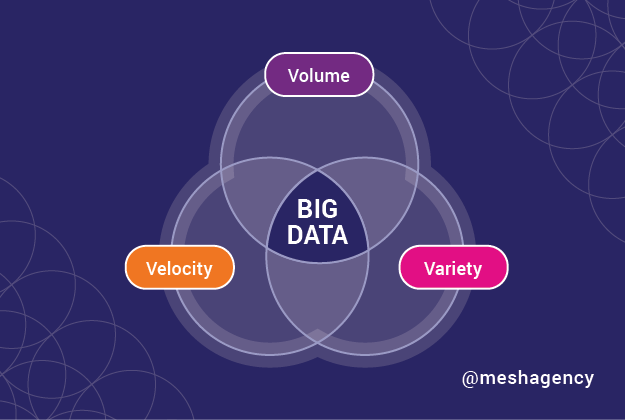
\includegraphics[height=6cm, angle=0,origin=c]{vvv.png}
	}
	\frame{\frametitle{VVV in astronomy}
		\begin{itemize}
			\uncover<1->{\item Volume: larger quantities of data by better facilitates }
			\uncover<2->{\item Velocity: Higher speed of getting data }
			\uncover<3->{\item Verity: More complex structures of data }
		\end{itemize}
	}
	%\subsection{Big telescopes}
	%\frame{
	%\frametitle{TMT}
	%}
	%\frame{
	%	\frametitle{JWST}
	%}
	%\subsection{Higher resolution}\frame{}
	%\subsection{Simulations}\frame{}
}
\subsection{Astronomical Surveys}
\frame{
	\frametitle{Sloan Digital Sky Server $\Rightarrow$ 40 TB}
	\centering
	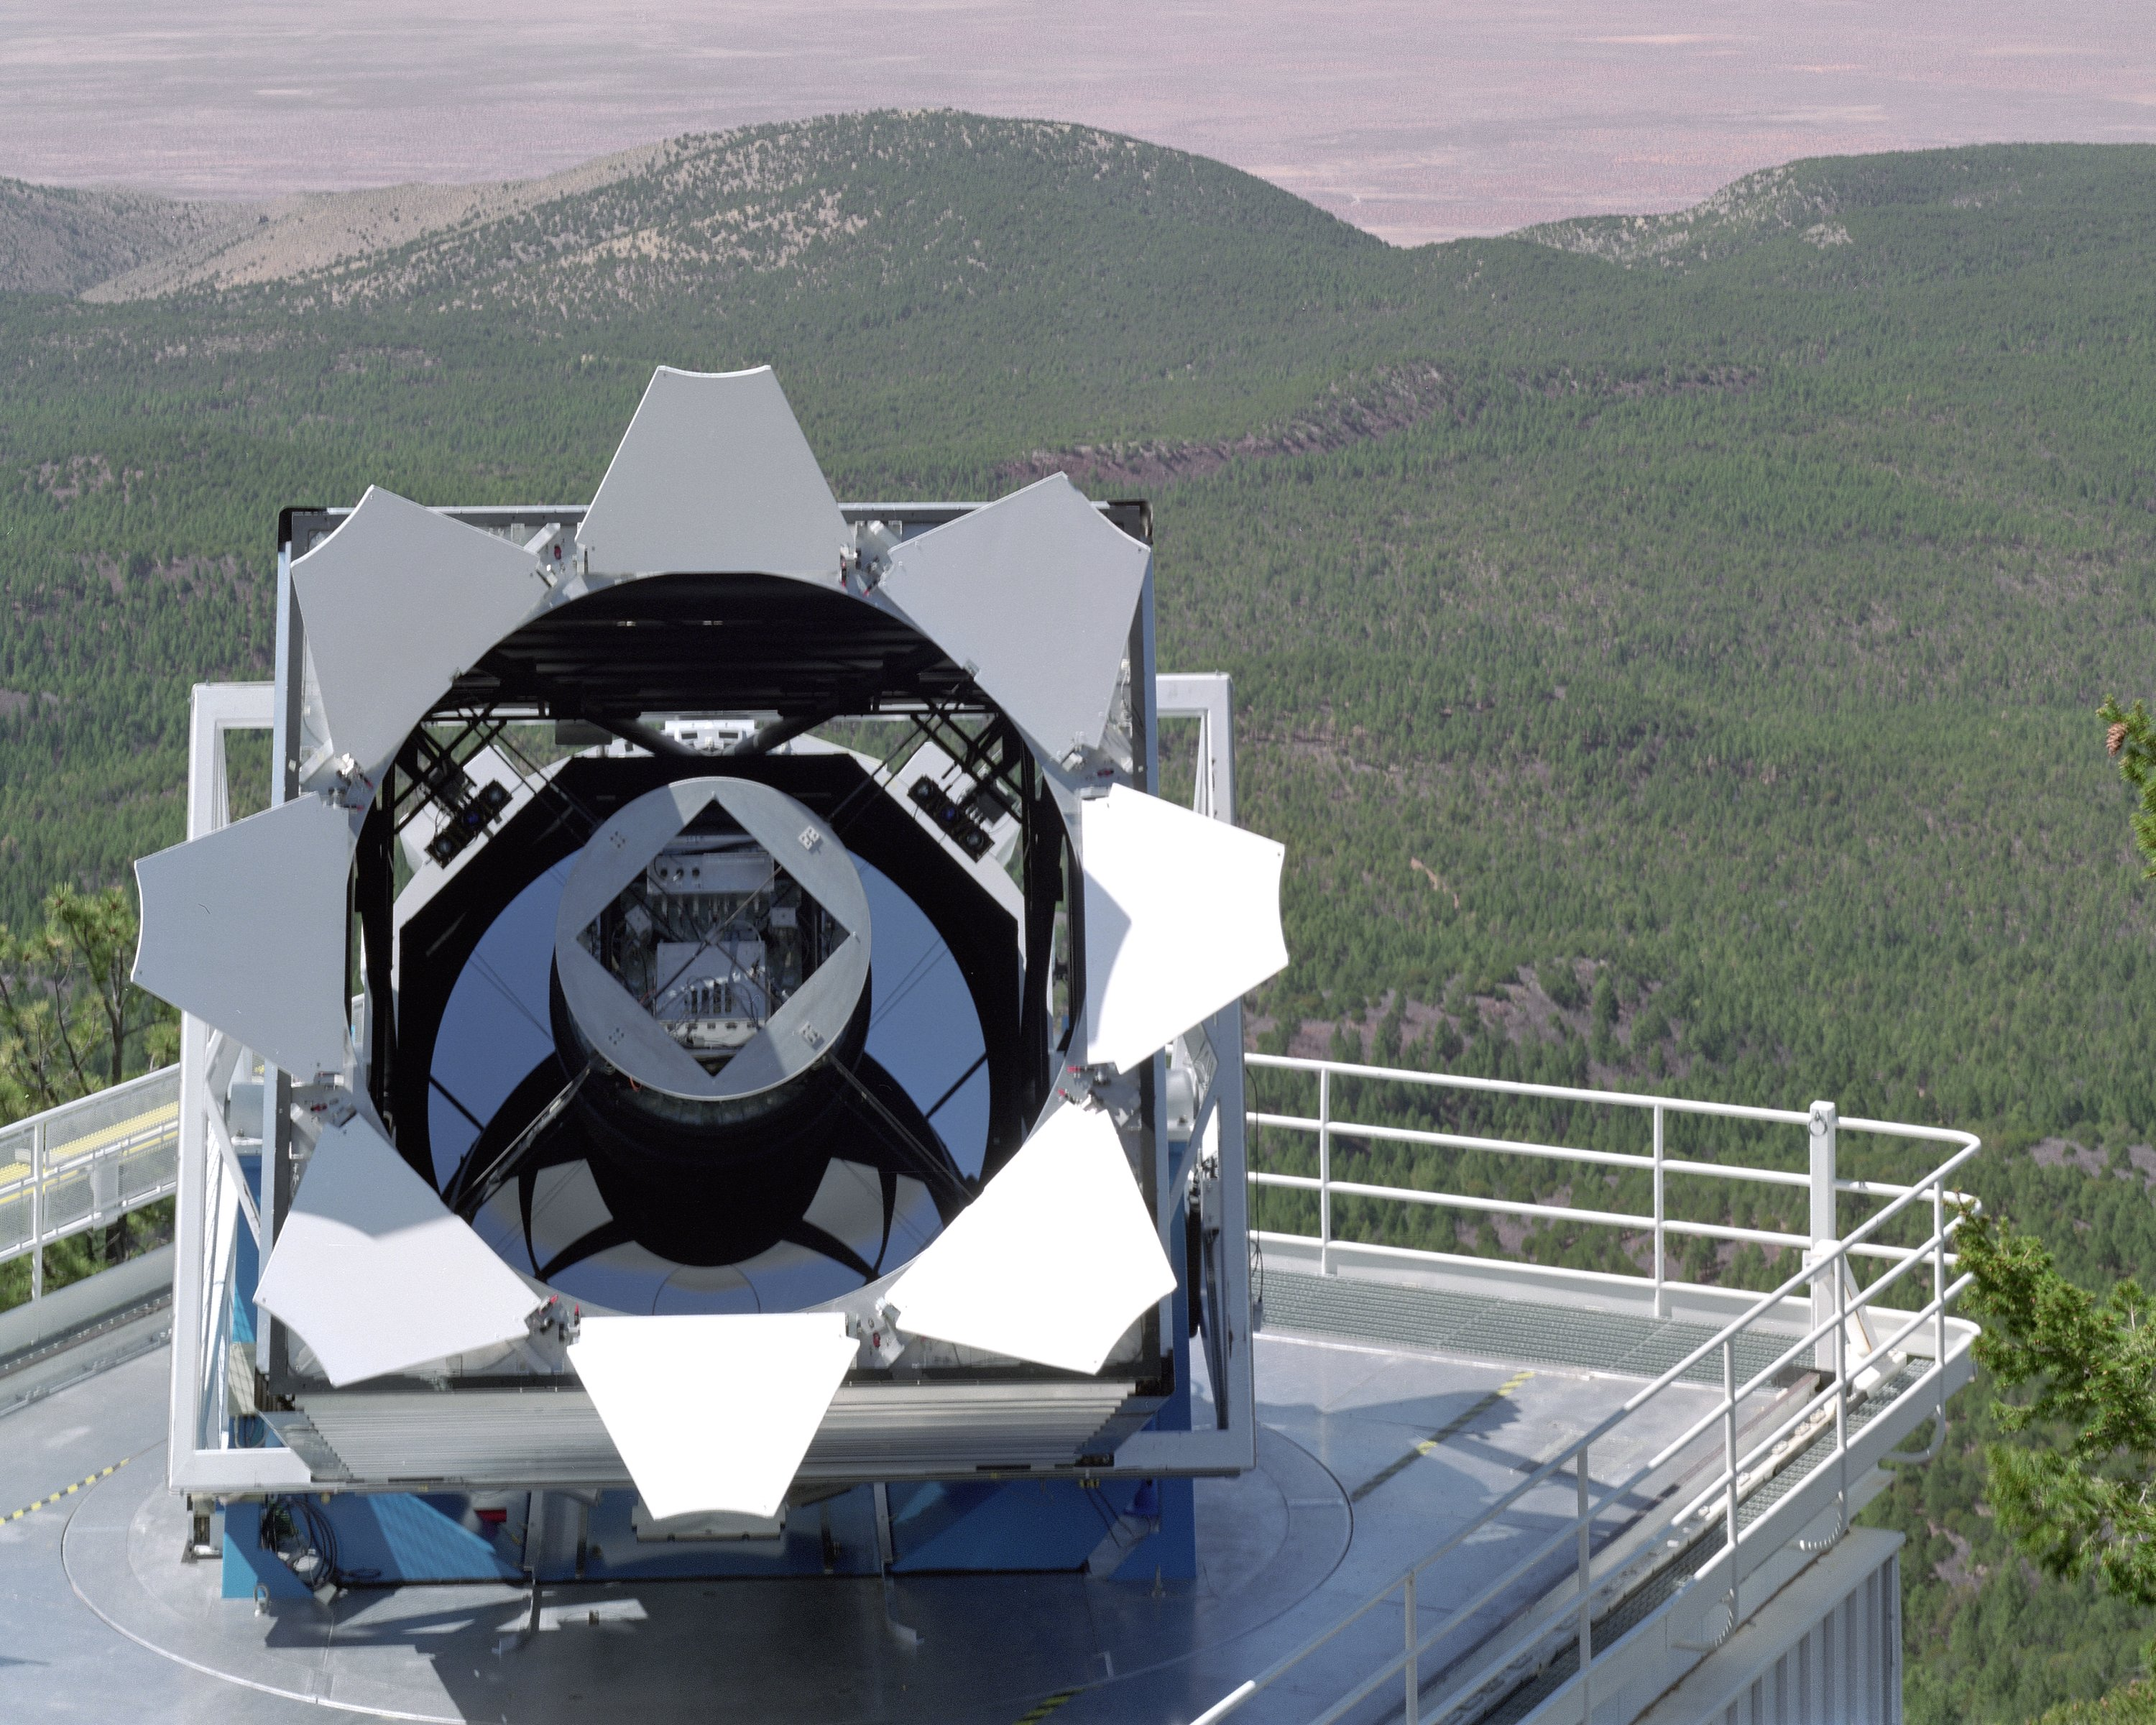
\includegraphics[height=6cm]{sdss-tel}
}
\frame{\frametitle{Sloan Digital Sky Server $\Rightarrow$ 40 TB}
\centering
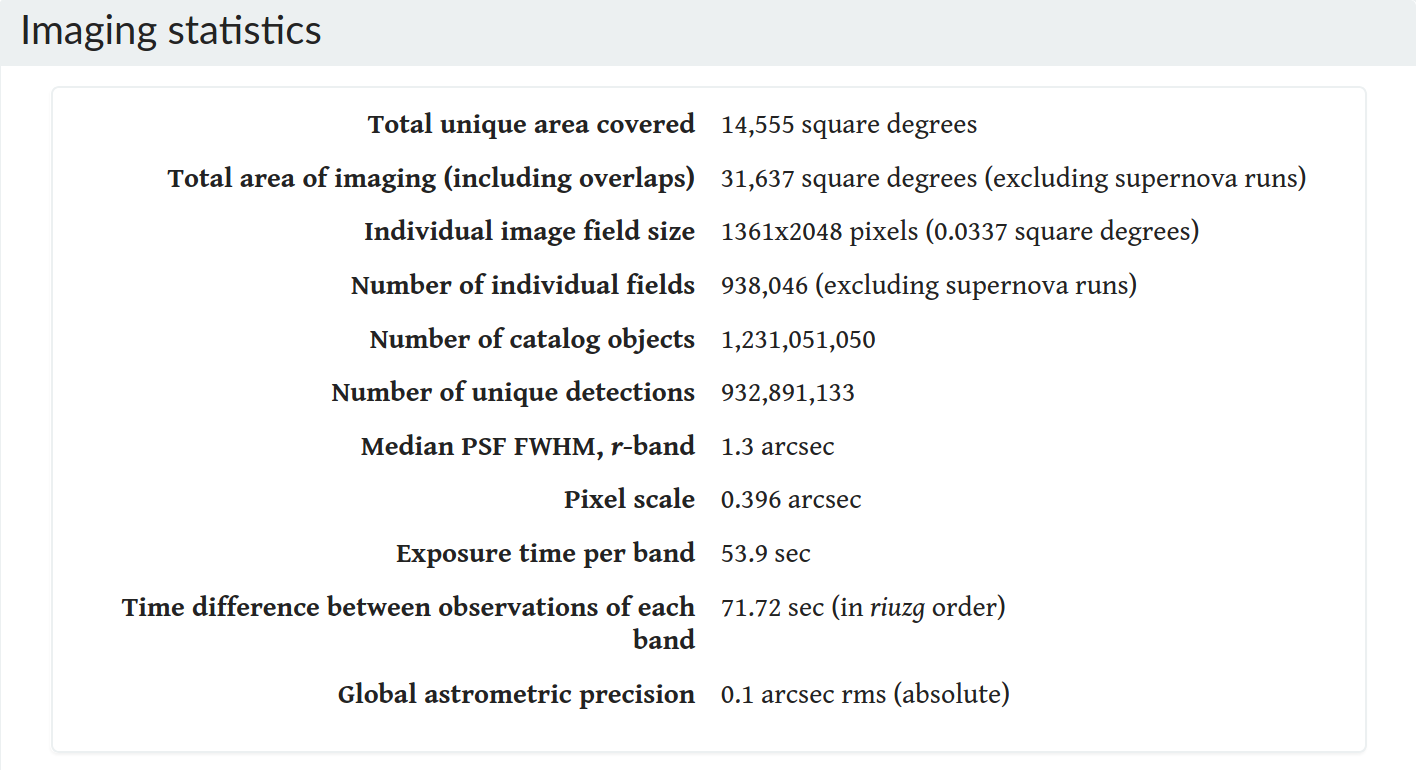
\includegraphics[width=\linewidth]{sdss-imaging-stat}

}
\frame{\frametitle{Sloan Digital Sky Server $\Rightarrow$ 40 TB}
	\centering
	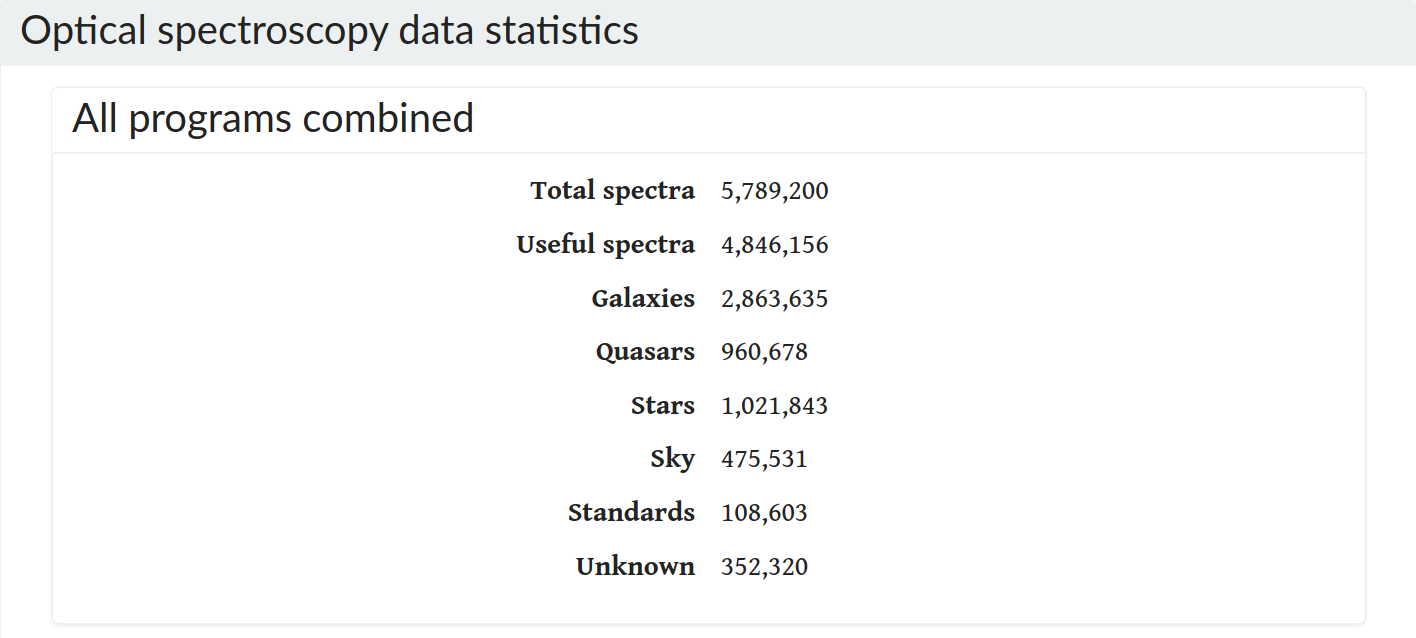
\includegraphics[width=\linewidth]{sdss-spec-stat}
	
}
\frame{\frametitle{Large Synaptic Survey Telescope $\Rightarrow$ 200 PB}
	\centering
	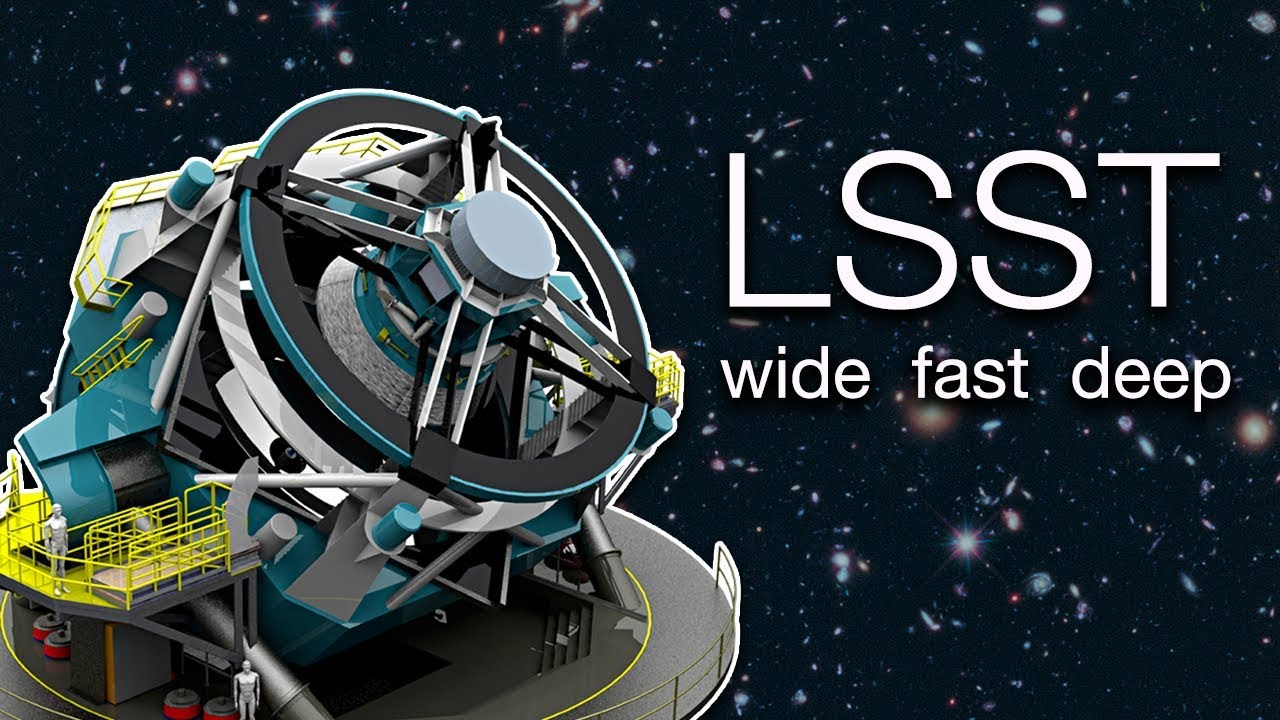
\includegraphics[height=6cm]{lsst}}

\frame{\frametitle{Large Synaptic Survey Telescope $\Rightarrow$ 200 PB}
\begin{itemize}
	\uncover<1->{\item 800+ panoramic images each night}
	\uncover<2->{\item 3.2 billion-pixel camera}
	\uncover<3->{\item Recording the entire visible sky twice each week}
	\uncover<4->{\item Each patch of sky will be visited 1000 times}
\end{itemize}}
\frame{
	\frametitle{Zwicky Transient Facility}
	\centering
	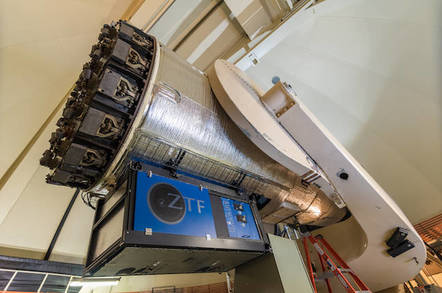
\includegraphics[height=6cm]{ztf_installed}
}

\frame{
	\frametitle{Zwicky Transient Facility}
	\centering
	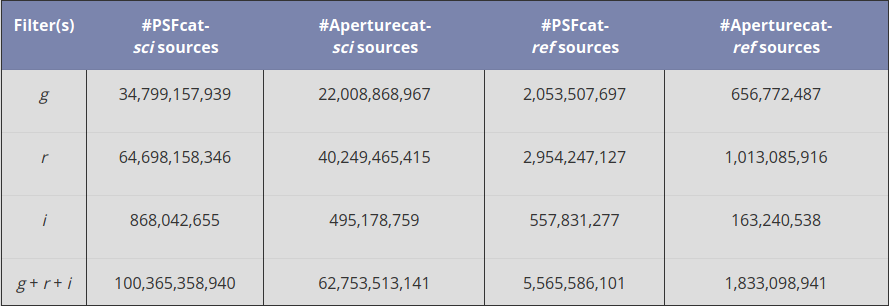
\includegraphics[width=\linewidth]{ztf-stat}
}


\frame{
	\frametitle{Dark Energy Spectroscopic Instrument}
	\centering
	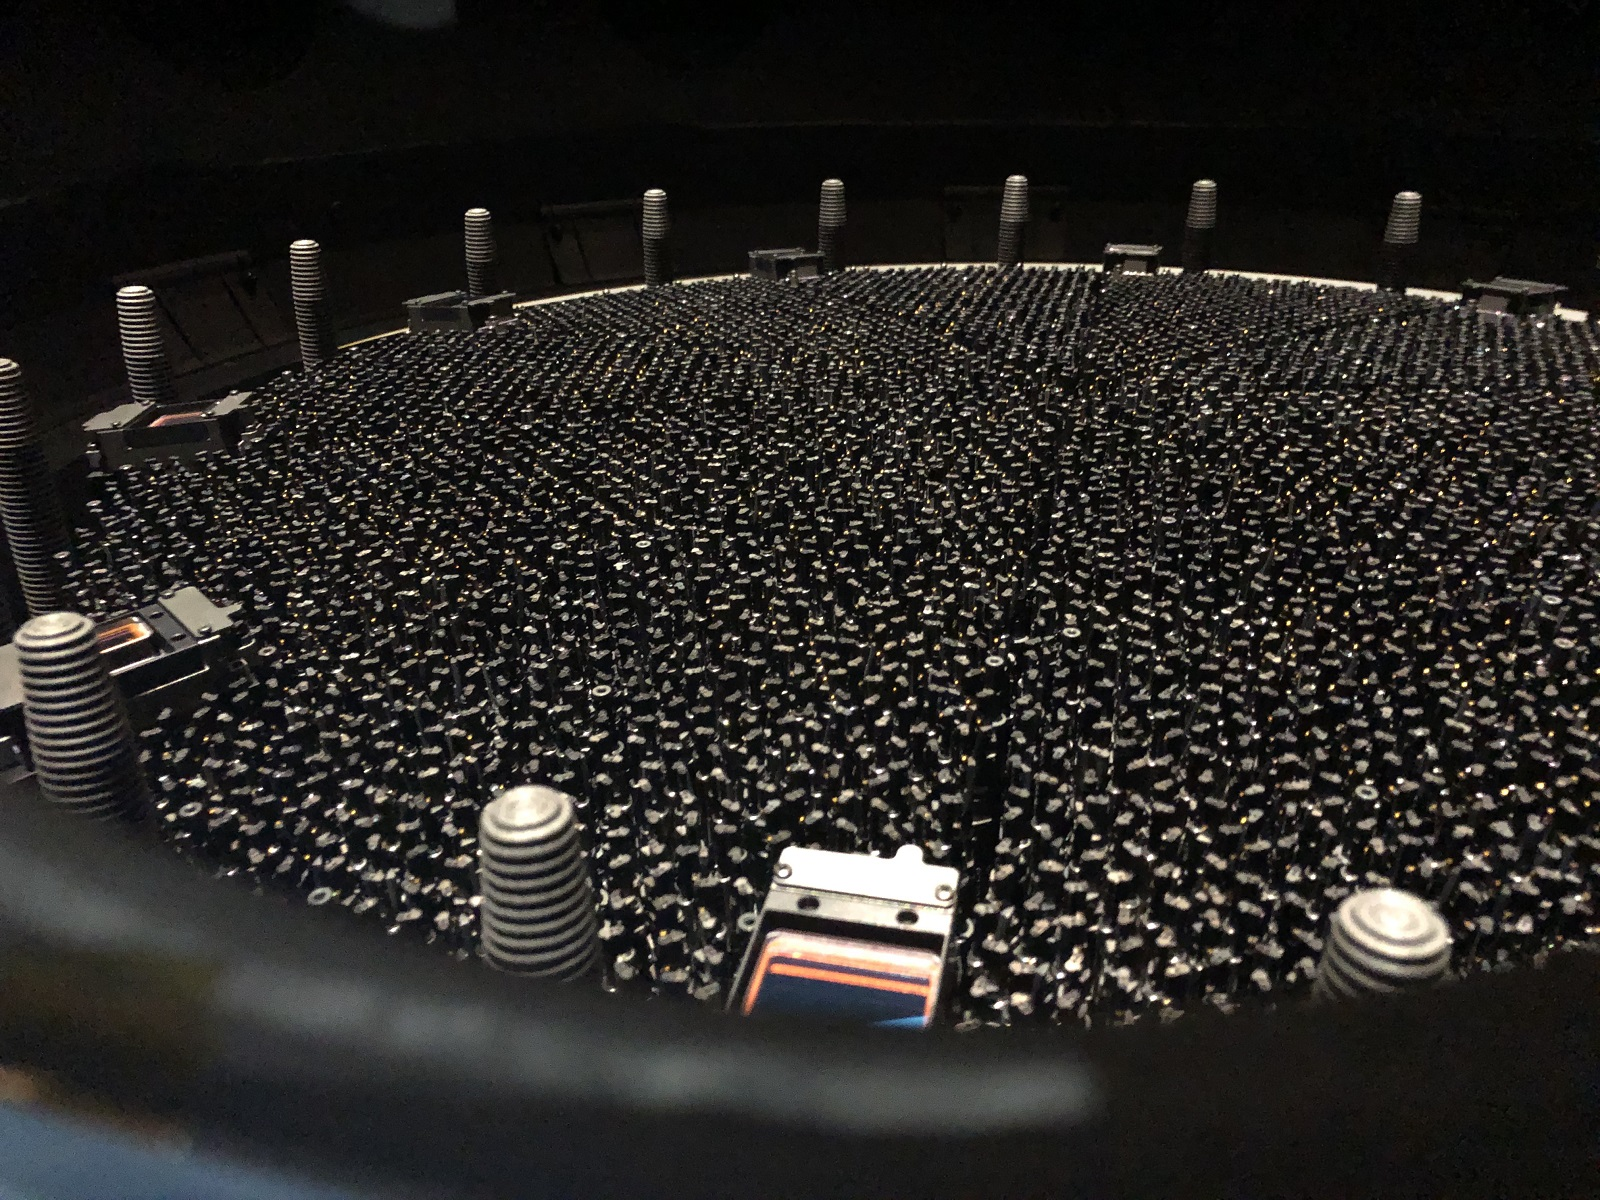
\includegraphics[height=4.55cm]{DESI_2}
	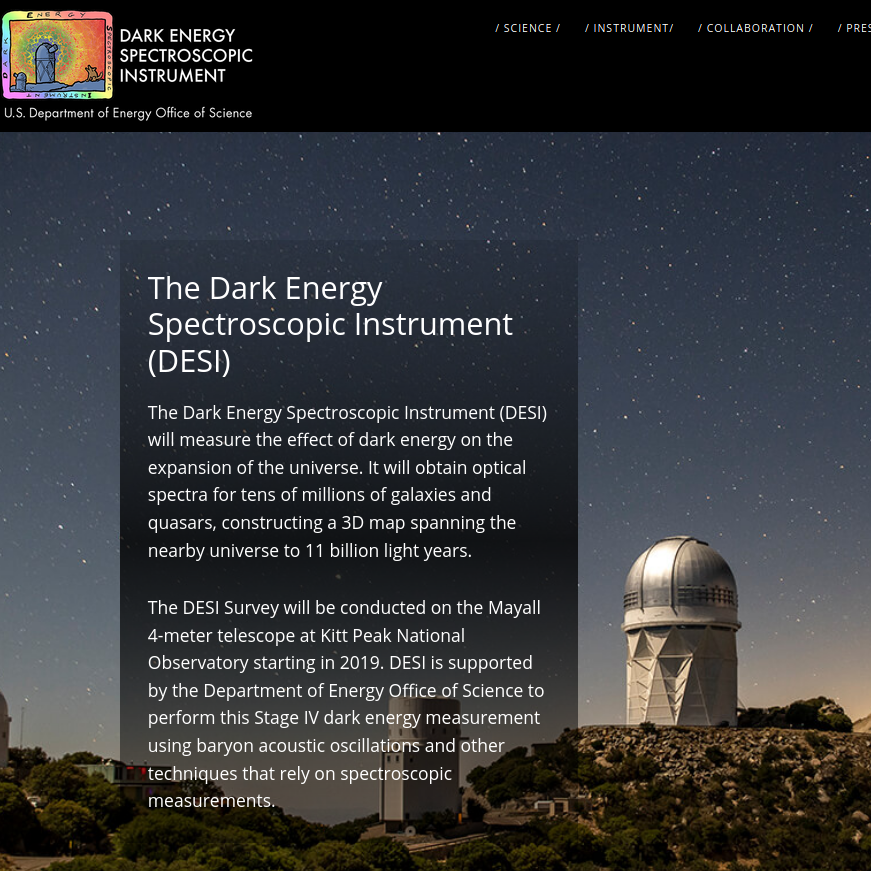
\includegraphics[height=4.55cm]{Desi}
}
\frame{
	\frametitle{Dark Energy Spectroscopic Instrument}
	\centering
	\Large{\begin{itemize}
\uncover<1->{\item Spectra of 25 M galxies, quasars, stars. }
\uncover<2->{\item 5000 spectra per exposure }
		\end{itemize}
	}
}
\frame{
	\frametitle{Square Kilometer Array $\Rightarrow$ 4.6 EB}
	\centering
	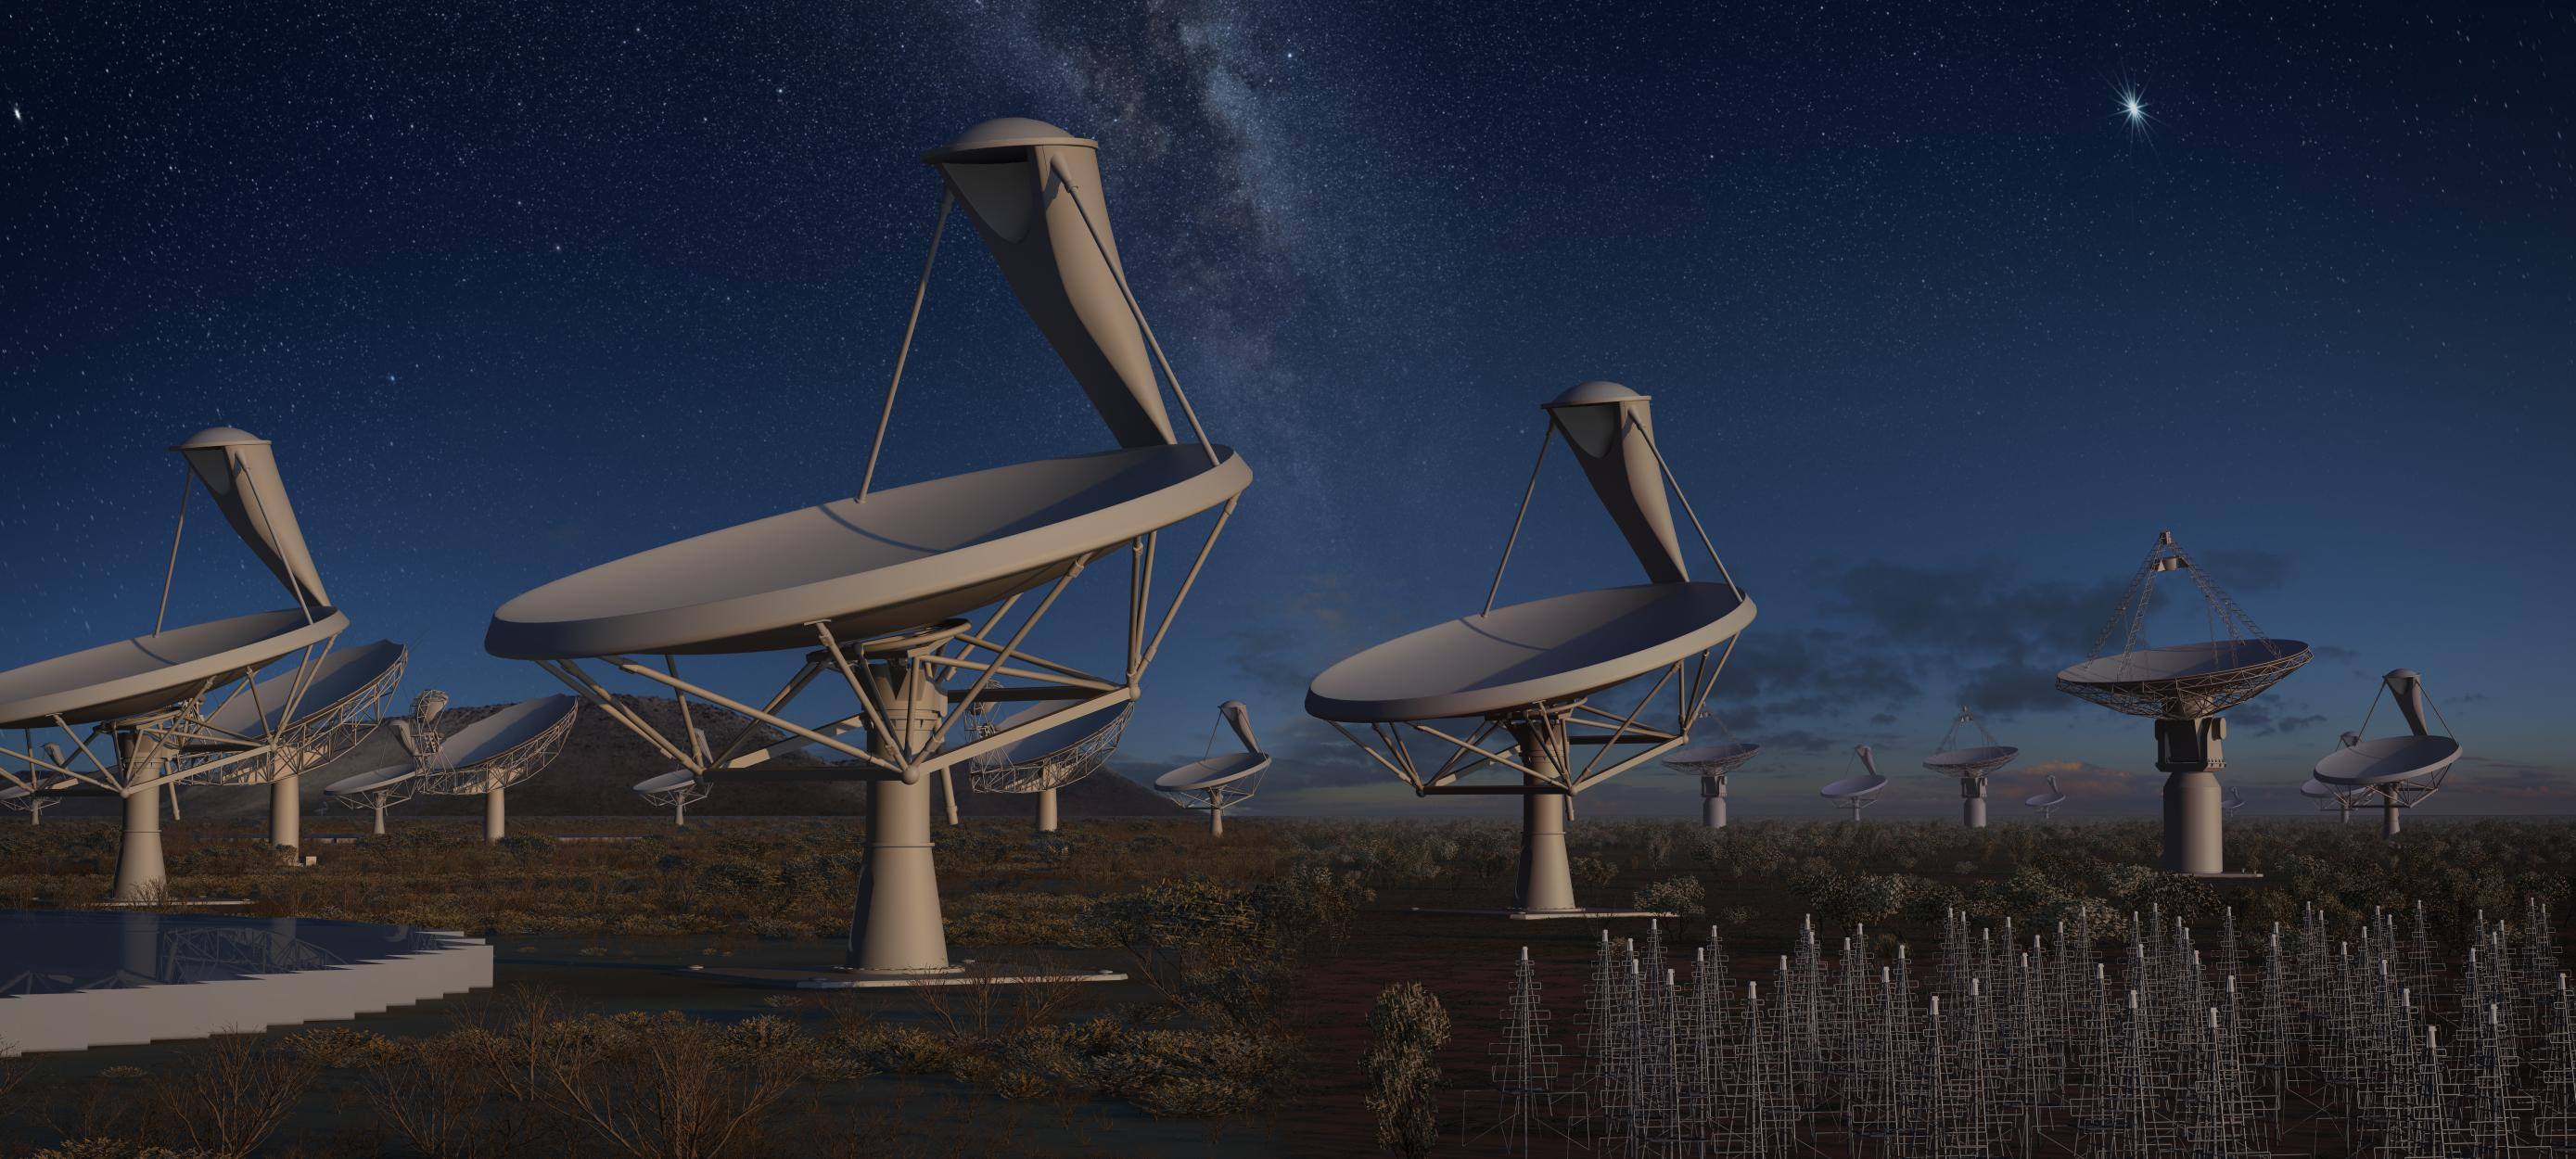
\includegraphics[height=5cm]{ska}
}

%\frame{\frametitle{Data volume} 
%\begin{table}[htbp]
%	\caption{}
%	\begin{tabular}{|l|c|}
%		\hline
%		\textbf{Sky Survey Projects} & \textbf{Data Volume} \\ \hline
%		SDSS & 40 TB \\ \hline
%		
%		LSST  & ~ 200 PB expected \\ \hline
%		SKA & ~ 4.6 EB expected \\ \hline
%	\end{tabular}
%	\label{}
%\end{table}
%
%
%
%}
\frame{ 
	\Large{
	\begin{block}

		\uncover<1->{Large surveys}
		\uncover<2->{$\Rightarrow$}
		\uncover<3->{Big Data}
		\uncover<4->{$\xRightarrow{ML}$ \\ }
		\uncover<5->{\centering Astronomy Knowledge}

	\end{block} }
}

%\frame{\frametitle{BIG DATA and ML}
%	
%	%	\begin{columns}[c]
%	%		\column{.5\textwidth}
%	%		\begin{center}
%	%			\includegraphics[scale=0.3]{}
%	%		\end{center}
%	%		\column{.5\texwidth}
%	%		\begin{center}
%	%			\includegraphics[scale=0.3]{} 
%	%		\end{center}
%	%	\end{columns}
%	
%	
%	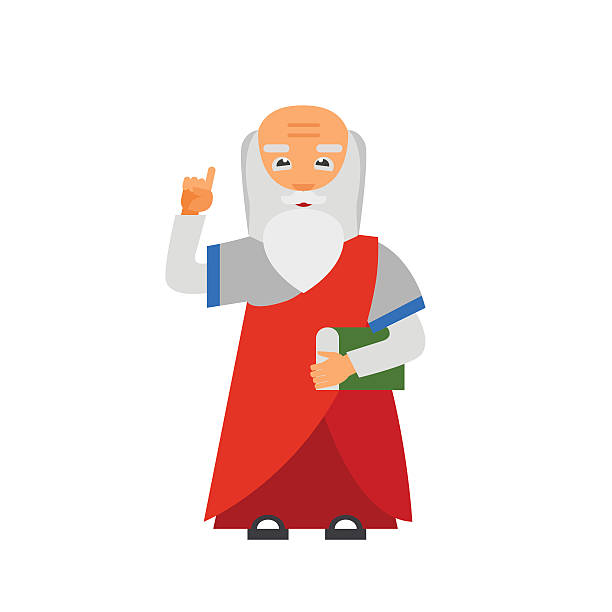
\includegraphics[width=0.5\linewidth]{old-wise.jpeg}
%		
\includegraphics[width=0.45\linewidth]{clumsy.jpeg}
% }


\section{ML Algorithms}{
\subsection{Overview}{
\frame{\frametitle{Supervised ML vs. Unsupervised ML	}
		\centering
	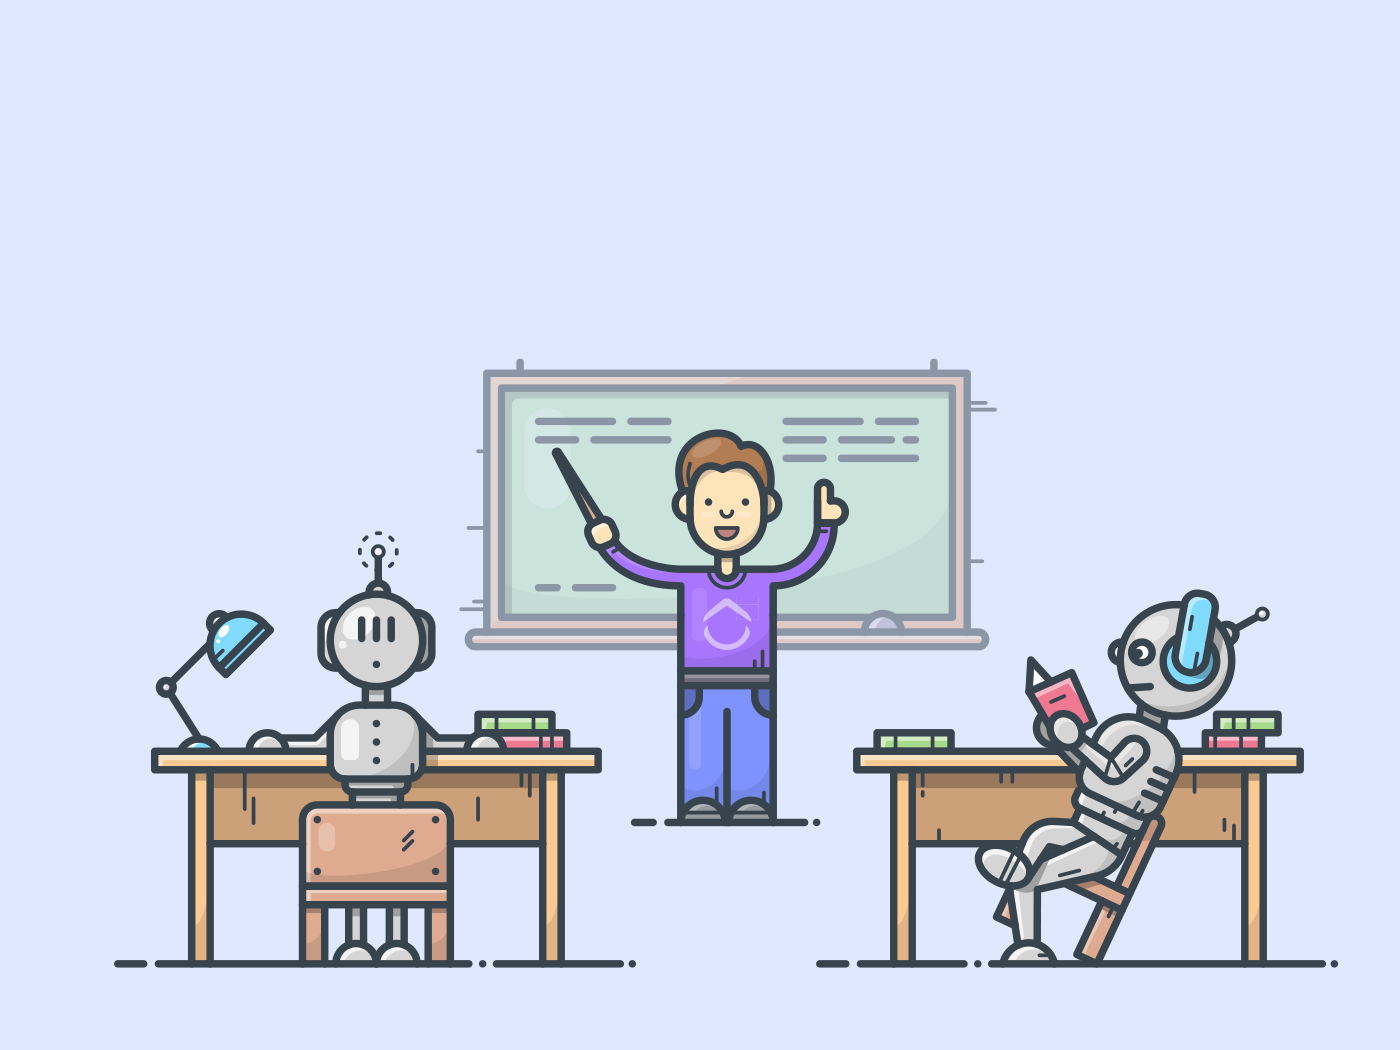
\includegraphics[width=0.8\linewidth]{external-content}
		}
	
\frame{\frametitle{Supervised ML vs. Unsupervised ML}
\begin{figure}
	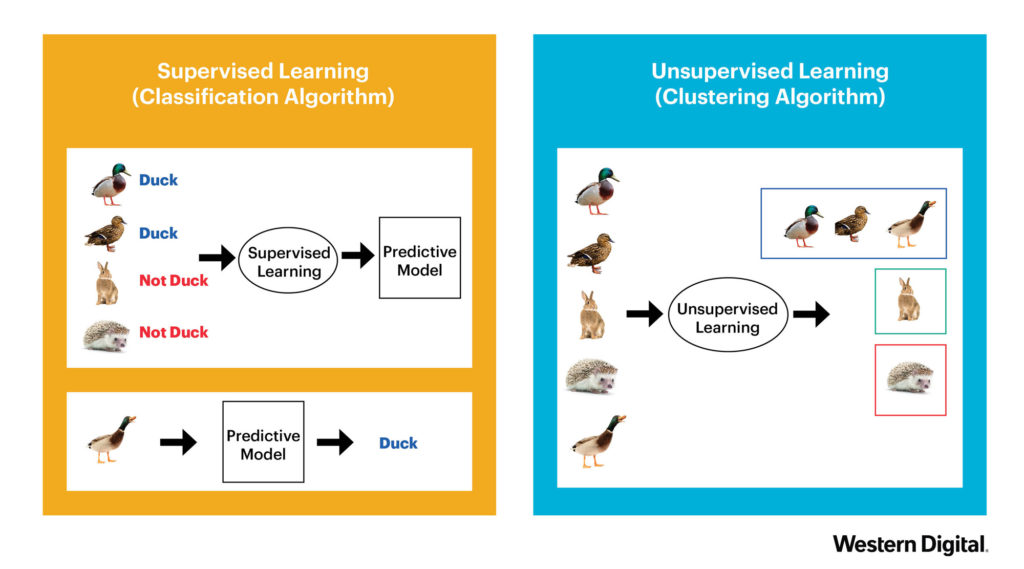
\includegraphics[width=\linewidth]{super.jpg}
%	\caption{}
%	\label{fig:example-supervised}
\end{figure}
}

}
\subsection{Supervised learning}
\frame{\frametitle{Stages of Supervised Learning}
	
	\begin{itemize}
		\uncover<1->{\item Training: 
			\begin{enumerate}
				\uncover<2->{\item Select a model }
				\uncover<3->{\item Set up hyper-parameters of model}
				\uncover<4->{\item Teach the machine by training set}
		\end{enumerate} }
		\uncover<5->{\item Validation: 
			\begin{enumerate}
				\uncover<6->{\item Change the hyper-parameters  }
				\uncover<7->{\item Select the optimum hyper-parameters}
		\end{enumerate} } 
		\uncover<8->{\item Testing: 
			\begin{enumerate}
				\uncover<9->{\item Test learned model by an unseen part of the data-set. }
				\uncover<10->{\item Select the best model and use it for predictions.}
		\end{enumerate} } 
	
		
	\end{itemize}
}

%\frame{\frametitle{Stages of Supervised Learning} 
%\centering
%\includegraphics[width=\linewidth]{.jpg}
%}

\frame{ \frametitle{Supervised Learning vs Traditional Model Fitting ?}

\uncover<1->{\begin{bclogo}{Similarities}
		\begin{itemize}
			\uncover<2->{\item Both need a set of labeled measurements and a model }
				
		\end{itemize} 
	\end{bclogo}}
\uncover<3->{\begin{bclogo}{Differences}
		\begin{itemize}
				\uncover<4->{ \item SML: model gets adapted by data}
				\uncover<5->{\item SML: model can be very nonlinear/complex }
				\uncover<6->{\item TMF: model is predefined and has limited adaptivity}
				\uncover<7->{\item SML: designed for predicting unseen data}
			\uncover<8->{\item TMF: infers  relationships between  features}
		\end{itemize} 
\end{bclogo}}	
}

\subsection{Unsupervised learning}{
\frame {\frametitle{How unsupervised learning works?}
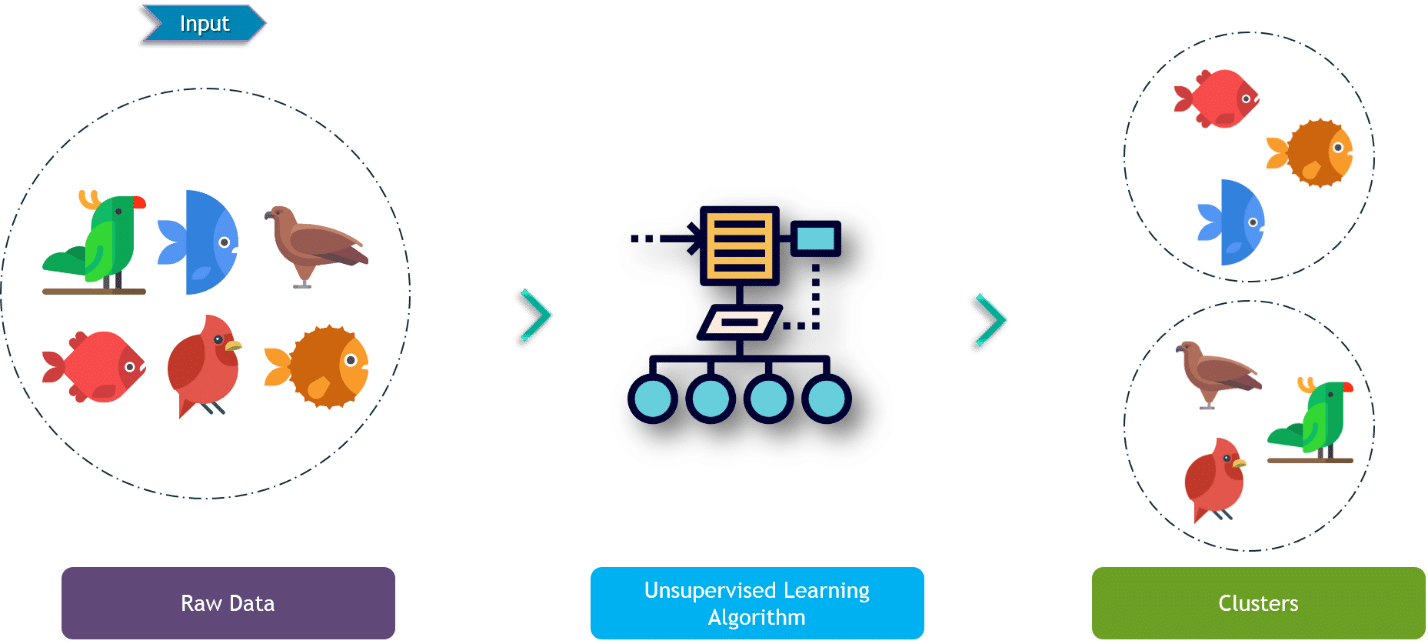
\includegraphics[width=\linewidth]{unsuper}}

\frame{\frametitle{Unsupervised Learning and knowledge discovery}
	\begin{itemize}
		\uncover<1->{\item Finding unknown patterns in the data set}
		\uncover<2->{\item Distinguishing similar and dissimilar objects  }
		\uncover<3->{\item Helping for visualization in lower dimensions }
		\uncover<4->{\item Recognizing odd objects (unknown unknowns)}
	\end{itemize}

\uncover<5->{\begin{block}{}
		\centering
		\huge{DATA $\xrightarrow{ML}$ Knowledge} 
		
 \end{block}}	
}


}




















\section{Supervised ML in astronomy}{

\subsection{Classification}\frame{}
\subsection{Regression}\frame{}
\subsection{Neural Network}\frame{}
}


\section{Unsupervised ML in astronomy}{
\subsection{Clustering}\frame{}
\subsection{outlier detection}\frame{}
\subsection{dimensionality reduction}\frame{}
\subsection{Neural network}\frame{text}
}

\section{ML and SKA}
\frame{}
\section{ML limitations}{ \frame{text}
\subsection{a}\frame{}
\subsection{b}\frame{}
}
\end{document}